% Autor: Alfredo Sánchez Alberca (email:asalber@ceu.es)
% Charts that shows the purpose of Statistics
\begin{tikzpicture}[every label/.style={text=color1}]
\tikzstyle{node} = [align=center, node distance=1cm, text=color1]; 
\tikzstyle{arrow} = [-latex, color2, line width=10pt];

\node (data) [label=-90:Data] at (0,1) {\includegraphics[height=1.5cm]{img/introduction/data.pdf}}; 
\pause
\node (information) [label=-90:Information] at (4.5,1)
{
\includegraphics[height=1.5cm]{img/introduction/information.png}}; 
\node at (2,1) [fill=color2,single arrow,shape border rotate=0,text=white, minimum width=1.1cm]{
\ STATISTICS\ \phantom{}};
\pause
\node (knowledge) [label=-90:Knowledge] at (9.5,1) {\includegraphics[height=1.5cm]{img/introduction/knowledge.png}};
\node at (7,1) [fill=color2,single arrow,shape border rotate=0,text=white, minimum width=1.1cm]{
Interpretation\phantom{}};
\pause
\node at (11.5,1) [fill=color2,single arrow,shape border rotate=0,text=white, minimum width=1.1cm]{
\ Decisions\ \phantom{}};
\end{tikzpicture} 